\chapter{Introduction} % Main chapter title

\label{ch_introduction} % Change X to a consecutive number; for referencing this chapter elsewhere, use \ref{Chapter1}

\todo{Add a short section about the significance of wind turbine failures and the advantages of using conditioning monitoring.}

%----------------------------------------------------------------------------------------
%	SECTION 1
%----------------------------------------------------------------------------------------
\section{System Overview}

The wind turbine that is analyzed in this thesis is part of the Cal Poly Wind Power Research Center.  This is designed for research into smaller wind turbines and to educate engineers in all aspects of the wind power industry.  The Cal Poly Wind Turbine Tower supports a 3 kW Horizontal-Axis Wind Turbine, and the tower was analyzed by Tae-gyun (Tom) Gwon\cite{Gwon_paper}.  In Gwon’s thesis paper, an ABAQUS model of the tower is developed to analyze natural frequencies and vibrations.  An FEM model, such as this one, is too complicated to run on a cheap microcontroller; however, the results of this model can be compared with the simple lumped-parameter model to determine the validity of the simplifications.

The Cal Poly Wind Turbine has no current method of detecting an imbalance.  It is possible to install an intrusive and expensive device that monitors all many tower parameters (such as multiple acceleration measurements at various positions on the tower and blades), but it would be much more desirable to have an inexpensive, device that can accurately detect an imbalance with zero to no setup/installation effort.

%----------------------------------------------------------------------------------------
%	SECTION 2
%----------------------------------------------------------------------------------------

\section{Objective}

The primary objective of this thesis is to develop a method for identifying a blade imbalance in the field.  This method must be simple enough to perform on a microcontroller in real time, while maintaining the ability to be mounted to any small scale wind turbine.   This will help to prevent any catastrophic failures resulting in damaged blades and an inoperable wind turbine.  Additionally, maintenance costs can be reduced because the turbines in good condition won't have to be inspected as often.  The main focus of the paper will be introducing a simplified turbine tower model and providing a digital signal processing method for analyzing the data.

A simplified tower model will help to develop and test various signal processing methods.  It is difficult and time consuming to obtain experimental data from the tower, so having a tower model will speed up the algorithm design process.  Once the signal processing method has been tested and refined on the analytic model, it can then be tested on experimental tower data will minimal tuning.

\section{Background}
Cal Poly’s wind turbine is in the Escuela Ranch in an unpopulated area.  The tower is a tapered tubular pole made of ASTM A572 Grade-50 Steel.  The tower has a tilting feature which allows relatively easy access to the nacelle.  The tower is rotated about 2 ball bearings at the base via a winch attached to the CPWPRC truck.  More details about the tower design and analysis can be found in \textit{Structural Analyses of Wind Turbine Tower for 3 KW Horizontal-Axis Wind Turbine} \cite{Gwon_paper}.

\section{Turbine Failures}
The goal of this project is to develop a method for detecting a rotor imbalance that could be potentially harmful to the turbine.  This would allow the turbine to be shut down before any failures occur.  

A common method for tracking and preventing turbine failures is the use of Supervisory Control and Data Acquisition (SCADA) alarms\cite{WT_failures_paper}.  SCADA is a control system architecture that uses high-level graphical user interfaces networked with peripheral devices (such as PLCs and PID controllers).  This is an effective method for predicting turbine failure, but can be expensive and complicated to implement.  An example of SCADA alarm results are shown in Figure \ref{fig:SCADA_table}.

\begin{figure}
	\centering
	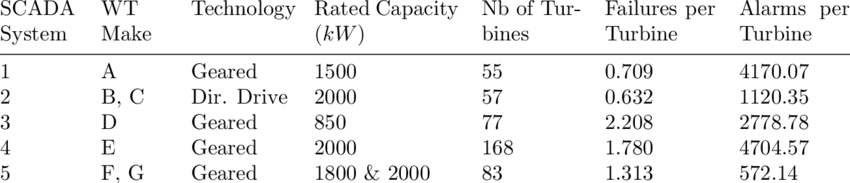
\includegraphics[scale=0.4]{SCADA_table}
	\decoRule
	\caption{Data used for the SCADA Alarms and Failure Analysis \cite{wind_turbine_failures}. \todo{Describe/explain the results in the SCADA table.}
}
	\label{fig:SCADA_table}
\end{figure}

According to a report on UK wind farms\cite{UK_turbine_failures}, there have been 1500 wind turbine-related accidents within 5 years.  Of those accidents, there were a total of 400 injuries to workers.  Many of these accidents are preventable if there is a reliable self-diagnosing system installed on the turbine.  This report also mentions incidents where ice has build up on the blades.  Most of these failures should be preventable if the rotor imbalance was detected right away and the turbine was shut down.


\section{Tower Vibration Research}
Wind turbine tower vibrations are important to the health of turbines and have been studied before.  In one study, a nonlinear state estimation technique\cite{NSET_vibration_modeling} (NSET) is used to attempt to predict wind turbine failures.  This model uses SCADA data to relate different operating parameters to the health of the turbine.  Figure \ref{fig:NSET_vibration_modeling_correlation} shows the correlation of power, wind speed, torque, blade angle, and tower vibration.  According to this paper, the tower vibrations are not enough information to predict turbine failures.

\begin{figure}
	\centering
	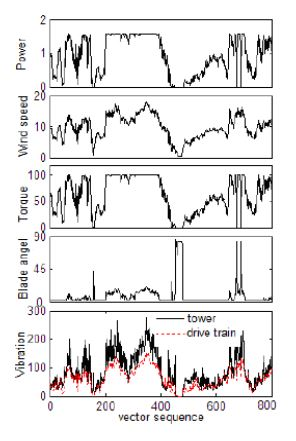
\includegraphics[scale=0.8]{NSET_vibration_modeling_correlation}
	\decoRule
	\caption{Correlation between different turbine parameters \cite{NSET_vibration_modeling}. \todo{get less blurry picture and add some more explanation.}}
	\label{fig:NSET_vibration_modeling_correlation}
\end{figure}

The research in \cite{NSET_vibration_modeling} attempts to detect \textit{any} turbine failure, while detecting only rotor imbalances may be slightly easier.

Most tower vibration analyses are empirically derived because of the stochastic nature of the wind speed and the amount of variables affecting the turbine.  Data-driven models\cite{data_driven_online_monitoring} are very common in the wind power space, especially with monitoring systems such as SCADA.

